\documentclass[UTF8]{article}
\usepackage{xcolor}
\usepackage{amsmath}
\usepackage{amssymb}
\usepackage{graphicx}
\usepackage{epstopdf}
\usepackage{inputenc}
\usepackage{geometry}
\usepackage{caption}
\geometry{left=2.5cm,right=2.5cm,top=2.5cm,bottom=2.5cm}

% For adding figures
\usepackage{graphicx}
\graphicspath{{./img/}}

% indenting paragraphs
\usepackage{changepage}

% for wrapping figure
\usepackage{wrapfig}

\usepackage[colorlinks=true, urlcolor=blue, linkcolor=red]{hyperref}

\begin{document}

\title{
  NavyRecordReview \\
  \large A Performance Summary Report Visualization Tool
}

\author{CDR Tom Gardner and CDR Chase Gruszewski}
\date{15 March 2024}
\maketitle


\begin{abstract}
NavyRecordReview (NRR) is a data visualization tool to streamline the process of
drawing insights from a Naval Officer's Performance Summary Record (PSR). It 
automatically converts the PSR's dense, tabular text into a rich, intuitive, 
and interactive display. All end-users of the PSR can benefit from 
NavyRecordReview's functionality, from an individual Officer preparing their
Letter-to-the-Board, to mentors conducting record reviews, to Apply Board Members 
preparing to brief a record in ``the tank." NavyRecordReview is available for 
use at \href{https://www.navyrecordreview.com}{www.NavyRecordReview.com}.
%\textcolor{red}{"dashboard"?}
\end{abstract}

\begin{figure}[h!]
 \centering
 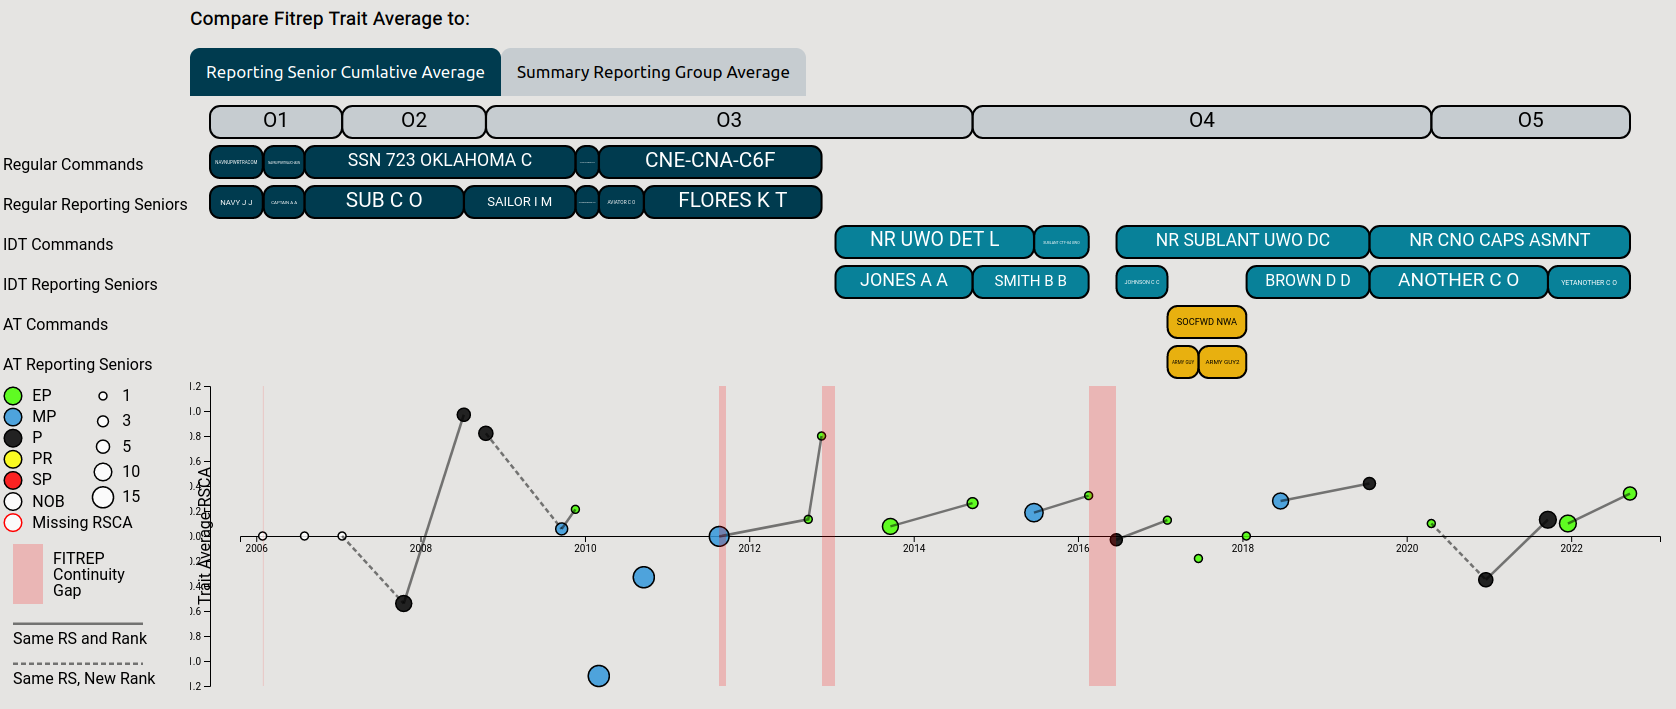
\includegraphics[width=0.75\textwidth]{nrr_dashboard.png}
 \caption{Sample NavyRecordReview PSR Visualization}
\end{figure}


\section{Background}
\subsection{The Problem}
NavyRecordReview was born in March 2021 while Tom was serving as an Assistant
Recorder for the Fiscal Year 2022 FTS/RES O-6/O-5/O-4 CONT URL Selection Boards.
Due to the ongoing Covid-19 pandemic, these Boards were consolidated and
conducted by a single group of Recorders and Members. Consequently, Tom spent an
entire month at the Bureau of Naval Personnel, much of which was spent
observing Members review and brief PSRs. This process struck Tom as wildly
inefficient, sometimes ineffective, and in all cases, ripe for improvement.\\

For anyone who participates in a Promotion or Apply Board, it quickly becomes apparent
that the goal of a Board Member's record review is to gain an understanding of
an Eligible's demonstrated performance and convey that understanding to the
other Board Members. This understanding comes not from personal knowledge of the
Eligible, but from reviewing documents in their official record - primarily the
PSR and Fitness Reports (FITREPs).\\

%The PSR (figure 2) is a table of column and rows of data summarizing all of the
%FITREPs an officer has recieved over the course of their career. 

Board Members perform tasks during record review that we categorize into two
types:
\textit{\textbf{rote}} and \textit{\textbf{expert}}. Examples of each follow:\\

\textit{\textbf{Rote}} tasks: 
\begin{itemize}
  \item Checking each FITREP for continuity with the previous FITREP.
  \item Comparing each FITREP Trait Average to the Reporting Senior's Cumulative
  Average (RSCA).
  \item Checking for Promotion Recommendations that ``break right."
  \item Checking for increasing Trait Averages among successive FITREPs from the
  same Reporting Senior while in the same Pay Grade. 
\end{itemize}

\textit{\textbf{Expert}} tasks: 
\begin{itemize}
  \item Evaluating career progression through demonstrated performance in
  demanding positions.
  \item Evaluating the comments in Block 41 of FITREPs to gain insight into 
  performance during specific periods of an Eligible's career.
  \item Deciding what elements of the applicable Community Brief the Eligible
  has satisfied and whether there may be any mitigating circumstances for
  shortcomings.
\end{itemize}

Tom watched Board Members diligently perform the rote tasks. He watched them 
painstakingly look for FITREP continuity gaps, mind-numbingly comparing thousands 
of dates, each written on different lines in MMDDYY format, to each other to see 
if there are any days in between, trying to keep straight how many days are in a
given month, what years contain leap days, etc. He watched them assiduously compare 
FITREP Trait Average to RSCA, often dozens of times per record. Let's just say, 
``mistakes were made," - Board Members are only human! - and it took days or weeks
longer than it should have. \\

A quick review of the verbs in the two lists of tasks above helps to demonstrate
what Tom felt watching the Members review records:\\

\begin{adjustwidth}{35pt}{35pt}

\indent \indent \textit{``Why are the 14 O-6s, 2 O-7s, and the O-9 who BUPERS brought
to Millington from around the world doing so much \textbf{checking} and
\textbf{comparing} of data when they should be focused on using their experience to
do more \textbf{evaluating} and \textbf{deciding} which records are the best?"}, and
\\

\indent \textit{``Why isn't the computer \textbf{automatically} checking for FITREP
continuity and whether the Trait Average is above or below RSCA?"}\\

\end{adjustwidth}

What's more, Members have to spend time doing what is refered to as
``arts \& crafts," drawing arrows and circles all over a PSR to indicate things like
missing continuity or Trait Averages above/below RSCA. What's \textit{even} more,
there was little standardization in the ``arts \& crafts" annotations. For example, Tom
observed 4 different ways that Members would indicate whether a FITREP's Trait
Average was above or below RSCA:

\begin{minipage}{0.7\linewidth}
\begin{itemize}
  \item Drawing an arrow from the higher number to the lower number,
  \item Drawing an arrow from the lower number to the higher number,
  \item Drawing a circle around the lower number,
  \item Drawing a circle around the higher number.
\end{itemize}
\end{minipage}
\hfill
\begin{minipage}{0.3\linewidth}
  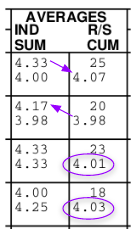
\includegraphics[width=0.4\linewidth]{inconsisent_annotations.png}\\
%  \captionof{figure}{Inconsistent ``arts \& crafts"}
%	Inconsistent ``arts \& crafts"
\end{minipage}


\pagebreak
The effect of the inconsistent ``arts \& crafts" was to impose unnecessary mental 
switching on Board Members. Each time a different Member stood up to brief a record,
everyone in ``the tank" had to reorient to a different set of annotation habits,
while trying to listen to the briefer speak. 


\subsection{The Solution}

After the first couple of days observing all of this as an Assistant Recorder, 
Tom started to look for ways to improve the process. It was clear that Members 
required a way to visualize the data contained in the PSR, along with features 
to automate many of the rote record review tasks, freeing them to focus on the 
expert tasks that only they can perform. Tom began sketching out various ways to
visualize PSR data. This took the form of a scatter plot with FITREPs 
represented as printed letters, displaying the Promotion Recommendation, on a 
horizontal axis representing time and a vertical axis representing the FITREP
Trait Average minus RSCA. \\

The first few attempts used hypothetical PSRs, resulting in an overly-simplistic
product. Feedback from Members and BUPERS staff was mixed, often skeptical that
it wouldn't work on ``a real record." So, Tom started sketching out the idea with
his own PSR. This is when he started to think the idea had promise.  \\

Armed with version 2.0 of the sketch, Tom found an opportunity to 
show it to RADM Andy Lennon, now RADM (ret.), who was in Millington serving on 
another Board. Tom had served previously with RADM Lennon and had a good feeling
that he would be interested in the idea. RADM Lennon liked the idea and asked if
he could show it to VADM Mustin, who was also in Millington at the time. The 
next day, RADM Lennon told Tom that VADM Mustin also liked the idea, which is
when Tom started coding a digital prototype.  \\ 


\begin{figure}[h!]
 \centering
 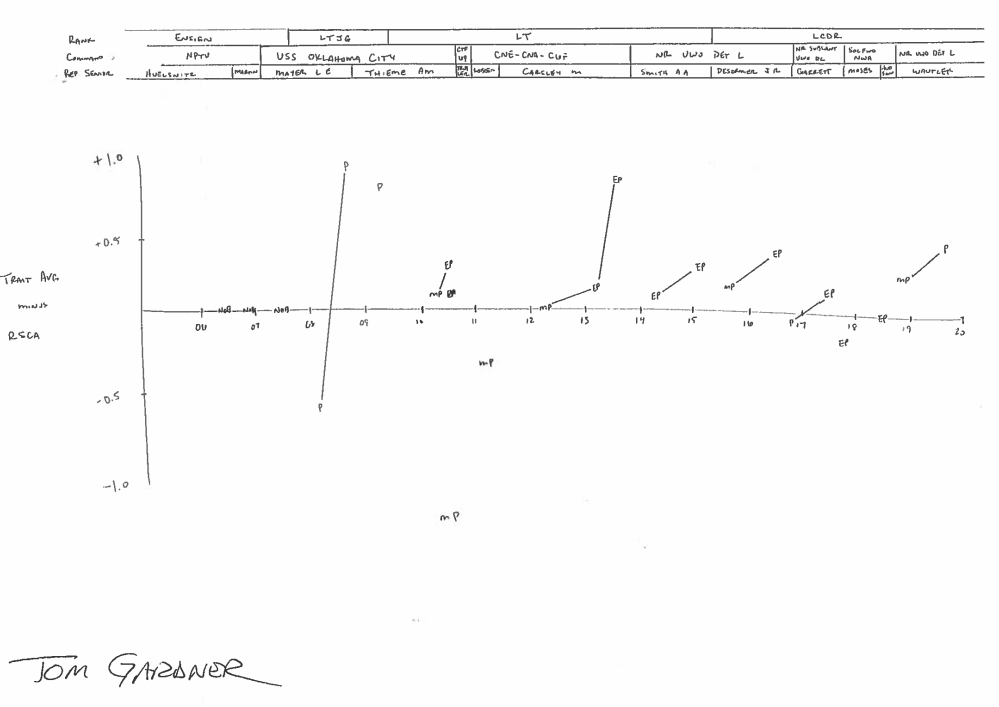
\includegraphics[width=0.95\textwidth]{original_sketch.png}
 \caption{Original Sketch of NavyRecordReview}
\end{figure}


\subsection{Implementation}

After coming off orders to Millington, Tom continued to develop the visualization
into a minimum viable product, which was newly hosted as a static website on
Github.com. Members of his Unit were a natural population of users for testing.
They could provide additional real-world PSRs as well as valuable perspective on 
the best ways to display information and handle edge cases. Chase, one of those
members of Tom's Unit, proved to be critically valuable to the project, with his
expertise and experience in programming, in general, and web development, in 
particular. \\

With Chase onboard, NavyRecordReview really started to take shape. Chase brought
renewed spirit to the project at times when it seemed to be stalling. Additionally, 
Chase's technical skills enabled implementation of critical features, such as
automatic PDF parsing, without which NavyRecordReview had a fatal data entry 
problem. \\

Shortly after Chase came onboard, we moved the site's hosting from GitHub to 
NavyRecordReview.com, where it remains today.

\section{Functionality}

\begin{itemize}
  \item \textbf{Automated Parsing:} The system will automatically render a 
  visualization by scanning a PSR PDF that Officers can download from the BUPERS
   On-Line website. While it says ``upload," this is a bit of a misnomer, as 
   nothing is ever sent to our servers and all code runs inside the user's 
   browser (ie ``client-side" processing).
  \item \textbf{Trait Average Comparision:} The system allows comparison of the 
  individual's trait average to the RSCA or the Summary Group Average, creating
  a contextual view of the individual's performance.
  \item \textbf{Performance Trend Lines:} Evaluations by the same Reporting 
  Senior, at the same Command, while the Officer is in the same Pay Grade are
  connected by solid trend lines, providing instant visual comparison of 
  comparable performance ratings over time. Evaluations by the same Reporting 
  Senior, at the same Command, \textit{but where the Officer has promoted 
  between Pay Grades} are connected by dashed lines.
  \item \textbf{FITREP Continuity Gap Identification:} Continuity gaps in an 
  indiviual's record are highlighted in red, quickly identifying any periods of
  time that might need to be addressed.
  \item \textbf{Manual Entry and Editing:} Records can be completely manually 
  entered, as well. The PSR table allows manual entry of performance data. 
  Additionally, this table can be used to correct errors in the PSR, such as 
  misspellings in the Command Name (discussed further in the Goals and Backlog 
  section).
  \item \textbf{Date Range Selection:} It's rare to need to review an 
  individual's entire record, so the ``Start Date" selector allows reviewers to
  zoom in on a specified period of time, making the individual's most recent
  performance trends more clear.
  \item \textbf{Multiple FITREP Comparison:} One of our newer features, this 
  allows multiple PSRs to be displayed at once. Reviewers can quickly toggle
  between PSRs by selecting the individuals name or view multiple records 
  side-by-side. In Multiview, records can either be compared across the past
  2 paygrades or the past 5 years.
\end{itemize}


\newpage

These features simplify and automate the process of marking up a PSR and result 
in a product that is more visually appealing and understandable:

\begin{figure}[h!]
  \centering
  \includegraphics[width=0.75\textwidth]{now_vs_future.png}
  \caption{Current PSR Markup vs. NavyRecordReview Visualization}
\end{figure}


\section{Use Cases}
Presently, we envision three distinct use cases:
\begin{enumerate}
  \item \textbf{Apply and Promotion Board Reviews:} The insipiration and primary purpose for the 
  project is to provide a better way to visualize the Trait Average performance 
  and Promotion Recommendations for an individual service member and assist with 
  assessing their historic level of performance. To be clear, this system is not 
  intended to replace the need for the human review of an individual service 
  record during a Board. It is intended to provide a clear assessment of the 
  discrete numerical information in a performance record including Promotion 
  Recommendations, Trait Averages vs. RSCA, Trait Averages vs. Summary Group 
  Averages, and performance trends across Reporting Seniors and Commands. This
  should free Board members' time in processing records to spend less time
  comparing numbers on a PSR and more time for reviewing the context (e.g. 
  Block 41 information), of the service member's performance.
  \item \textbf{Reporting Senior Assessments:} By their very nature, FITREPs are 
  comparative evaluations, with the burden of assessing which individuals are 
  most suitable for promotion placed on the Reporting Senior. In assessing each 
  Summary Groups ranking, Reporting Seniors not only assess performance for the 
  period of report, but also the overall suitablility of the individual for 
  promotion which may include additional factors such as time-in-grade, history 
  of performance, history of assignments, additional qualification, and more. To 
  provide Reporting Seniors with and additional tool to assess these additional 
  factors, the NavyRecordReview provides the option to upload multiple PSRs from
  individuals and see them compared side by side, saving time and providing a
  graphical representation of these additional factors that may assist in ranking
  personnel within a Summary Group.
  \item \textbf{Individual Record Reviews:} By extension of use cases 1 and 2, the
  ability for individuals and mentors to get a quick snapshot of career 
  performance is valuable when preparing for Boards or mapping out future
  waypoints in their career. NavyRecordReview provides the opportunity for 
  Boards, Reporting Seniors, and the individual to all share the same graphical
  view of the individual's performance throughout their career.
\end{enumerate}


\section{Goals and Backlog}
While there are multiple prospective benfits for different end users on this project, our goal remains to move the visualization tools into a BUPERS rowned platform so that the visualization can be used to improved process for the Apply Board, and eventually, statutory Promotion boards.

Additionally, in our efforts to continuously improve the NavyRecordReview PSR Visualization 
Project, we've worked with fellow Sailors, human resource experts, 
Flag Officers, and BUPERS staff. Some of the main items in our current goals 
list include:
\begin{itemize}
  \item \textbf{Improved Aesthetics:} Presently, the project operates on a 
  functional, no frills design. While useable, it is not particularly 
  delightful to use. We intend to improve the appearance of the project by 
  enhancing the table (below the graph) to match the PSR PDF that is generated
  by BUPERS, and simplify the process for making edits. Additionally, we intend
  to expand the FAQ section and instructional information to offer users
  resources to help understand how they can assess PSRs using the tool. In our
  more ambitious moments, we'd like to run user testing with a cohort of ~10 x 
  O-6s to see how they interact with the system and what UI/UX changes could be
  made to improve the experience for this user group.

  \item \textbf{Data Smoothing:} In the development of this project, we've found
  that it's very common for an individual's PSR to contain minor variances from
  year to year that can confuse the graphical representation of the data.
  Generally these include minor variances in the spelling/abbreviation of a 
  Command name, primary duty, or Reporting Senior title. Presently, these 
  mistakes can be corrected using the program's manual editting feature to
  correct the data. This works, but can be time consuming. To help improve the 
  user experience, we intend to offer automated data smoothing, where the 
  program will look for spellings that are very close together and offer 
  ``did you mean..." suggestions.

  \item \textbf{Expand Applicability:} A glaring drawback of NavyRecordReview in
  its current form is that it only works on Officer's performance records, which
  ignores roughly 85\% of the members of the US Navy. If the Navy were to show 
  interest in this type of digital modernization of record review, we want to 
  expand functionality to cover Enlisted records.

  \item \textbf{Direct PSR Parsing:} Currently, the program builds a PSR 
  assessment by scanning PSR PDF and looking for information at specific 
  coordinates on the PDF. To date, this has worked reliably, but it is a 
  ``brittle" solution -- meaning that a small change in the way the PSR PDF's are
  styled/generated could break the entire system and require an update.
  Ideally, we'd want the PSR visualization system to be integrated into BOL's 
  suite of tools, where it could directly pull data points from the 
  individual's record and use the information to populate the graph. This goal 
  depends on adoption by the Navy and partnership with BUPERS to implement the
  system.

\end{itemize}


\end{document}


